\chapter{维护和维修}

维护维修工作务必严格遵守本手册的所有安全指示。

维护、校准、维修工作必须根据最新的服务手册进行操作,服务手册可以在官网 \url{https://lebai.ltd} 上查看。

维修必须由授权服务商或本公司指定的专业技术人员进行。必须确保维护维修工作规定的安全级别,遵守有效的国家或地区的工作安全条例,同时应检测所有的安全功能是否正常。

维护维修工作的目的是为了确保系统正常运行,或在系统故障时帮助其恢复正常状态。维修包括故障诊断和实际的维修。

操作机器人或控制箱时必须遵循以下安全程序和警告事项:

\innerinfo{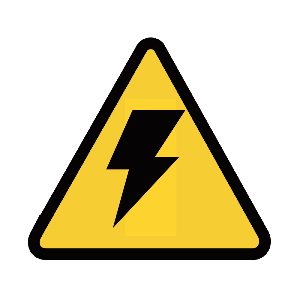
\includegraphics[width=1.8cm]{image/19.pdf}
\\
\includegraphics[width=1.8cm]{image/20.pdf}
}{}{\begin{itemize}
\item 维修时需要采取必要的预防措施以避免其他人在维修期间重新接通系统电源。断电之后仍要重新检查系统,确保其断电;
\item 重新开启系统前请检查接地连接;
\item 严禁用户自行拆卸机器人或控制箱;
\item 乐白指定服务商或专业技术人员维修时请遵守ESD(静电释放)法规;
\item 避免水或粉尘进入机器人或控制箱。
\end{itemize}}

\innerinfo{
\includegraphics[width=1.8cm]{image/20.pdf}
\\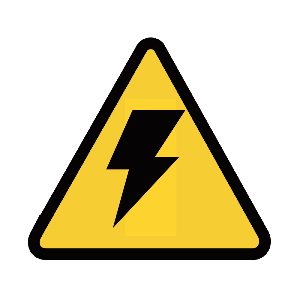
\includegraphics[width=1.8cm]{image/19.pdf}
}{}{\begin{itemize}
\item 禁止改变软件安全配置中的任何信息。如果安全参数变更,整个机器人系统应被视为新系统,这就意味着所有安全审核过程,比如风险评估,都必须更新。
\item 使用部件号相同的新部件或本公司批准的相当部件替换故障部件。
\item 该工作完成后立即重新激活所有禁用的安全措施。
\item 将所有维修操作记录下来,并保存在整个机器人系统相关的技术文档中。
\item 控制箱没有最终用户可自行维修的零件。如果需要维护或维修服务,请联系您的经销商或本公司。
\end{itemize}}
